\documentclass[11pt, english]{article}
\usepackage{graphicx}
\usepackage[colorlinks=true, linkcolor=blue]{hyperref}
\usepackage[T1]{fontenc}
\usepackage[utf8x]{inputenc}
\usepackage{listingsutf8}
\usepackage[spanish]{babel}
\selectlanguage{spanish}
\usepackage[svgnames]{xcolor}
\usepackage{booktabs}

\usepackage{listings}
\usepackage{afterpage}
\pagestyle{plain}

\definecolor{dkgreen}{rgb}{0,0.6,0}
\definecolor{gray}{rgb}{0.5,0.5,0.5}
\definecolor{mauve}{rgb}{0.58,0,0.82}

%\lstset{language=R,
%    basicstyle=\small\ttfamily,
%   stringstyle=\color{DarkGreen},
%    otherkeywords={0,1,2,3,4,5,6,7,8,9},
%    morekeywords={TRUE,FALSE},
%    deletekeywords={data,frame,length,as,character},
%    keywordstyle=\color{blue},
%    commentstyle=\color{DarkGreen},
%}

\lstset{frame=tb,
language=Java,
aboveskip=3mm,
belowskip=3mm,
showstringspaces=false,
columns=flexible,
numbers=none,
keywordstyle=\color{blue},
numberstyle=\tiny\color{gray},
commentstyle=\color{dkgreen},
stringstyle=\color{mauve},
breaklines=true,
breakatwhitespace=true,
tabsize=3,
inputencoding=utf8/latin1,
extendedchars=true,
literate={á}{{\'a}}1 {é}{{\'e}}1 {ó}{{\'o}}1 {ú}{{\'u}}1 {ü}{{\"u}}1 {ñ}{{\~n}}1 {¿}{{?`}}1 {¡}{{!`}}1
}

\usepackage{here}


\textheight=21cm
\textwidth=17cm
%\topmargin=-1cm
\oddsidemargin=0cm
\parindent=0mm
\pagestyle{plain}

%%%%%%%%%%%%%%%%%%%%%%%%%%
% La siguiente instrucción pone el curso automáticamente%
%%%%%%%%%%%%%%%%%%%%%%%%%%

\usepackage{color}
\usepackage{ragged2e}

\global\let\date\relax
\newcounter{unomenos}
\setcounter{unomenos}{\number\year}
\addtocounter{unomenos}{-1}
\stepcounter{unomenos}
\gdef\@date{ Curso  2018 / \arabic{unomenos}}

\begin{document}

\begin{titlepage}

\begin{center}
\vspace*{-1in}
\begin{figure}[htb]
\begin{center}
\includegraphics[width=10cm]{../res/pics/logo.jpg}
\end{center}
\end{figure}

\vspace*{0.4in}
\begin{large}
\textsc{Procesadores de Lenguaje}:\\
\end{large}
\vspace*{0.2in}
\begin{Large}
\textbf{\textsc{Nombre de nuestro lenguaje}} \\
\end{Large}
\vspace*{0.3in}
\begin{large}
\@date\\
\end{large}
\vspace*{0.3in}invalid utf-8 byte sequence spanish characters listing latex
\rule{80mm}{0.1mm}\\
\vspace*{0.1in}
\begin{large}
Realizado por: \\

Medina Medina, David Alberto  \\
Brito Ramos, Christian  \\
Hernández Delgado, Christopher \\
López González, Néstor \\
\vspace*{0.3in}
\end{large}

\includegraphics[width=3cm]{../res/pics/LogoEscuela.jpg}
\end{center}
\end{titlepage}

\newcommand{\CC}{C\nolinebreak\hspace{-.05em}\raisebox{.4ex}{\tiny\bf +}\nolinebreak\hspace{-.10em}\raisebox{.4ex}{\tiny\bf +}}
\def\CC{{C\nolinebreak[4]\hspace{-.05em}\raisebox{.4ex}{\tiny\bf ++}}}

\tableofcontents
\newpage

\section{Definición del lenguaje (Autor: Quien termine antes)}
Introducir breve introducción del lenguaje que planteamos.
\newpage

\subsection{Tipos de datos (David)}
Cualquier leguaje de programación necesita definir un conjunto de \emph{tipos de datos}, esto es, la batería de valores y operaciones que puede adquirir una variable. Cada tipo de dato está definido en el lenguaje por un \emph{literal} único que lo representa, lo que permite que cada tipo de dato tenga un representación física específica.

Los tipos de datos definidos en el lenguaje son los que figuran en el \emph{cuadro \ref{tab:table1}}. Las características críticas de implementación que define a cada tipo son:

\begin{description}
	\item[Entero] Representa a todas y cada una de las variables enteras que sean declaradas en el lenguaje. Este tipo de dato presenta un tamaño de 4 bytes (32 bits) y permite representar números enteros con signo. El \emph{complemento a 2} es el sistema elegido para definir el signo del número entro. Este dato se representa por el literal \texttt{int}. El rango de valores que puede tomar es 
	
	\begin{equation}\label{eq:equation1}
		\left [-2^{N-1},\: 2^{N-1}-1 \right ] = \left [-2^{32-1},\: 2^{32-1}-1 \right] = \left [-2147483648,\: 2147483647 \right]
	\end{equation}
	
	donde, $N$ es el número de bits disponibles para representar el número el número entero (32 bits).
	\item[Coma flotante de simple precisión] Este tipo de dato representa número reales en coma flotante de simple precisión con un tamaño de 4 bytes (32 bits) siguiendo el estándar \emph{IEEE 754}. En la figura \ref{fig:figure1} puede observarse como esta representación binaria los bits se organizan en tres sectores principales:
	\begin{itemize}
		\item \textbf{Signo} (1 bit). Se trata de un sólo bit que define el signo del número: positivo (0) o negativo (1).
		\item  \textbf{Exponente (8bits)}. Se trata de un número entero con signo de complemento a 2 ($\left [ -128,\: 127\right ]$)
		\item \textbf{Mantisa (23 bits)}. Conforma la fracción a la derecha de la coma binaria y un bit de encabezado implícito.
	\end{itemize}
	Este tipo de dato se representa con el literal \texttt{real}. Su rango de valores es de $\left [ 1.18 \cdot 10^{–38},\; 3.4 \cdot 10^{38} \right ]$.
	\begin{figure}[H]\label{fig:figure1}
		\centering
		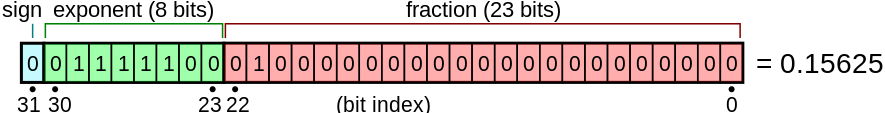
\includegraphics[width=0.75\textwidth]{../res/pics/data-types/float_diag.png}
		\caption{Representación binaria de número en coma flotante de simple precisión (\emph{IEEE 754})}
	\end{figure}

	\item[Caracter] Este tipo de dato es usado para representar caracteres de codificación \emph{UTF-8}, es por este motivo que el tamaño de que ocupan las variables de tipo caracter son de 4 bytes siendo \texttt{char} el literal que lo representa.
	\item[Booleano] Se trata de un tipo de dato utilizado para representar representar valores booleanos. Su tamaño es de 1 bit, por lo que tan solo puede tomar dos valores: \texttt{1} (verdadero) ó \texttt{0} (falso). El literal que lo representa es \texttt{bool}.
\end{description} 

\begin{table}[h!]
	\begin{center}
		\caption{Tipos de datos}
		\label{tab:table1}
		\begin{tabular}{l|l|l|l}
			\toprule
			\textbf{Tipo} & \textbf{Literal} & \textbf{Tamaño} & \textbf{Rango}\\
			\midrule
			Entero & int &4 Bytes & $\left [-2147483648,\: 2147483647 \right]$\\
			Coma flotante de simple precisión & real & 4 Byte & $\left [ 1.18 \cdot 10^{–38},\; 3.4 \cdot 10^{38} \right ]$\\
			Caracter & char & 1 Byte & \emph{UTF-8}\\
			Lógico & bool & 1 Bit & $\left [0,\; 1 \right ]$\\
			\bottomrule
		\end{tabular}
	\end{center}
\end{table}

En el siguiente ejemplo se muestra cómo se declaran las variables con los literales de los tipos descritos anteriormente:

\lstinputlisting[language=C++]{../res/lst/data-types/data-type.x}

\subsection{Colecciones de datos: \texttt{Arrays}}
Las variables pueden ser agrupadas en colecciones de datos de una dimensión denominados \emph{arrays}. En este lenguaje, cualquier tipo de dato puede formar parte de un \emph{array}.

% Añadir listado de ejemplo
\newpage

\subsection{Palabras reservadas (Christian)}
Aquí va el texto. Poner siempre un código de ejemplo.
\newpage

\subsection{Comentarios (Christian)}
Aquí va el texto. Poner siempre un código de ejemplo.
\newpage

\subsection{Tipos de operadores}
Aquí va el texto. Poner siempre un código de ejemplo.

\subsubsection{Operadores aritméticos (David)}
Aquí va el texto. Poner siempre un código de ejemplo.

\subsubsection{Operadores lógicos (Christopher)}
Aquí va el texto. Poner siempre un código de ejemplo.

\subsubsection{Operadores bit a bit (Christian)}
Aquí va el texto. Poner siempre un código de ejemplo.

\subsubsection{Operadores de array (Néstor)}
Los operadores de arrays nos permiten realizar operaciones con arrays, tratándolos como a subconjuntos. Los operadores a definir son los siguientes:
\begin{description}
	\item [Unión] La unión de dos arrays consiste en crear un nuevo array formado por los elementos del primer array y los del segundo.
	\item [Diferencia] La  diferencia de un array con otro consiste en crear un nuevo array con todos los elementos del primer array, descartando aquellos que aparecen en el segundo.
	\item [Intersección] La intersección de dos arrays consiste en crear un nuevo array formado por todos los elementos comunes entre el primer y el segundo array.
	\item [Concatenación] La Nuevo array formado por los elementos del primero seguido de los del segundo.
\end{description}
\begin{table}[h!]
	\begin{center}
		\caption{Tipos de operadores de arrays}
		\label{tab:table3}
		\begin{tabular}{c|c|c}
			\toprule
			\multicolumn{1}{c}{\textbf{Operador}} & \multicolumn{1}{c}{\textbf{Símbolo}} & \multicolumn{1}{c}{\textbf{Formato}}
			\\ \midrule
			UNIÓN                            & U                        & \{ARR\} U \{ARR\}
			\\ \midrule
			DIFERENCIA                             & D             & \{ARR\} D \{ARR\}
			\\ \midrule
			INTERSECCIÓN                            & I                            & \{ARR\} I \{ARR\}
			\\ \midrule
			CONCATENACIÓN                            & +                            & \{ARR\} + \{ARR\}
			\\ \bottomrule
		\end{tabular}
	\end{center}
\end{table}

A continuación mostramos un ejemplo de uso de los operadores de array para un caso trivial meramente ejemplificativo:
\begin{lstlisting}[frame=single]
int[6] a = new int[6]{0,1,2,3,4,5}
int[7] b = new int[7]{3,4,5,6,7,8,9}

int[] c = a U b ..c = {0,1,2,3,4,5,6,7,8,9}
int[] d = a D b ..d = {0,1,2}
int[] e = a I b ..e = {3,4,5}
int[] f = (a U b) D (a I b) ..f = {0,1,2,6,7,8,9}
int[] g = d + f + a ..g = {0,1,2,0,1,2,6,7,8,9,0,1,2,3,4,5}
\end{lstlisting}
\newpage

\subsection{Estructuras de control}
Aquí va el texto. Poner siempre un código de ejemplo.

\subsubsection{Sentencias \texttt{if-ifelse-else} (Néstor)}
La estructura de control if-ifelse-else sentencia condicional que está compuesta de los siguientes bloques:
\begin{description}
	\item[Bloque \texttt{if}] Este bloque está identificado por la siguiente estructura:
	\begin{equation}\label{eq:if}
	\{Expr\}\;?:
	\end{equation}
	En caso de ser verdadera, se ejecutarán las instrucciones que van seguidas de la expresióm \ref{eq:if}. Sólo puede existir un único bloque \texttt{if} al principio de una sentencia \texttt{if-ifelse-else}.
	\item[Bloque \texttt{ifelse}] Si no se cumple la condición del bloque anterior, se comprueba si la condición de este bloque se cumple para posteriormente ejecutar el conjunto de instrucciones que se encuentran en su contexto. En caso contrario, pasa a ejecutarse el siguiente bloque \texttt{elseif} La estructura de este bloque es el siguiente:
	\begin{equation}\label{eq:if}
	.\;\{Expr\}\;?:
	\end{equation}
	\item[Bloque \texttt{else}] Si ninguna de la expresiones de los bloques anteriores cumple la condición, se ejecutarán las instrucciones contenidas en este bloque. La estructura de este bloque es la siguiente:
	\begin{equation}\label{eq:if}
	.?:
	\end{equation}
	Sólo puede existir un único bloque \texttt{else} al final de una sentencia \texttt{if-ifelse-else}.
\end{description}

\begin{lstlisting}[frame=single, caption=Ejemplo de uso de la sentencia \texttt{if-ifelse-else}]
int a = 25
int b = 0

a > 20 ?:
	b = a - 10
. a < 10 ?:
	b = a + 5
.?:
	b = -1
\end{lstlisting}

\subsubsection{Bucle \texttt{for-forelse-else} (Christopher)}
Aquí va el texto. Poner siempre un código de ejemplo.

\subsubsection{Bucle \texttt{while-whileelse-else} (Christian)}
Aquí va el texto. Poner siempre un código de ejemplo.
\newpage

\subsection{Funciones (David)}
Aquí va el texto. Poner siempre un código de ejemplo.
\newpage

\subsection{Funciones primitivas (Néstor)}
En nuestro lenguaje, Van a existir predefinidas un conjunto de funciones primitivas que facilitarán al programador su trabajo en el desarrollo del programa. Las funciones están divididas en las siguientes categorías:

\begin{description} 
	\item [Interacción entrada-salida] Las funciones básicas de E/S son: 
	\begin{description}
		
		\item[\texttt{bool print(T salida)}] Esta función permite mostrar por pantalla el valor de \texttt{salida}, cuyo tipo \texttt{T} puede ser \texttt{int, real, bool, char} o una string (\texttt{char[]}). Si la operación termina correctamente la primitiva devolverá \texttt{true}, en caso contrario, devuelve \texttt{false}.
		\item[\texttt{bool scan(char[] entrada)}] Esta rutina permite leer el valor pasado por teclado una vez se pulse \texttt{ENTER} (\texttt{0x0D}). Si la operación termina satisfactoriamente la primitiva devolverá \texttt{true}, en caso contrario, devuelve \texttt{false}.
	
		\begin{lstlisting}[caption=Ejemplo de uso de la función \texttt{print()} y \texttt{scan()}]
		int number
		char[] name
		print("Introduzca el primer número: ")
		a = scan()
		print("¿Cuál es su nombre? ")
		name = scan()
		print("El usuario " + name + " ha introducido el número " + number)
		\end{lstlisting}
	\end{description}


	\item [Funciones para arrays numéricos] Las funciones para arrays numéricos permiten operaciones que impliquen el uso de arrays de enteros, números en coma flotante o combinar ambos tipos. El tipo \texttt{T} de las siguientes funciones indica que el tipo del parámetro de entrada o el tipo de retorno de la función puede ser \texttt{int} o \texttt{real}:
	
	\begin{description} 
		\item [\texttt{int length(array)}] Devuelve el número de elementos del array.
		\item [\texttt{T sum(array)}] Devuelve la suma de todos los elementos contenidos en el array.
		\item [\texttt{T res(T[] array)}] Devuelve el resultado de restar todos los elementos del array.
		\item [\texttt{real prod(T[] array)}] Devuelve el producto de todos los elementos contenidos en el array.
		\item [\texttt{int prod(T[] array1, T[] array2)}] Devuelve el producto escalar de los dos arrays.
		\item [\texttt{real coc(T[] array)}] Devuelve el cociente de todos los elementos contenidos en el array.
		\item [\texttt{T[] append(T[] array, T[] element, int position)}] Coloca en la posición \texttt{position} del array un elemento que debe ser del mismo tipo que el resto del array. Los demás elementos a partir de la posición especificada serán desplazados una posición a la derecha.
Se devuelve la referencia al array resultante.
		\item [\texttt{T[] delete(T[] array, int position)}] Elimina el elemento de la posición \texttt{position} del array y devuelve la referencia al array resultante. Los demás elementos a partir de la posición especificada serán desplazados una posición a la izquierda. 
		\item [\texttt{T[] find(array,element)}] Devuelve una referencia a un array de enteros, que representan las posiciones donde se encuentra un elemento en el array.
		\item [\texttt{T[] sort(T[] array, T[] ascendent)}] Devuelve la referencia a un array con los elementos ordenados de forma ascendente si \texttt{ascendent} es igual a \texttt{true}; en caso contrario, los ordenará de forma descendente.
		\item [\texttt{bool equal(T[] array1, T[] array2)}] Devuelve \texttt{true} si los dos arrays son iguales en tamaño y los elementos están dispuestos en el mismo orden. En caso contrario, devuelve \texttt{false}.
	\end{description} 
\end{description} 

\begin{lstlisting}[frame=single, caption=Ejemplo de uso de funciones primitivas para arrays numéricos]
int[] v1 = {2,5,9,5}		
int[] v2 = {5,4,8,9,3}		
int tam = length(v1)		..tam = 4
int n1 = sum(v1)			..n1 = 21
int n2 = sum(v2)			..n2 = 29
int[] v3 = sum(v1,v2)		..v3 = {7,9,17,14,3}
int[] v4 = res(v1,v2)		..v4 = {-3,1,1,-4,-3}
int n3 = prod(v1)			..n3 = 450
int n4 = prod(v2)			..n4 = 4320
int[] v5 = prod(v1,v2)		..v5 = {10,20,72,45,0}
int[] v6 = coc(v3,v2)		..v6 = {2,5,9,5,0}
float[] v7 = coc(v1,v2)		..v7 = {0.4,1.25,1.125,0.5555555556,0.0}
append(v1,6,3)				..v1 = {2,5,6,9,5}
delete(v1,3)				..v1 = {2,5,9,5}
int[] found1 = find(v1,5)	..found1 = {2,4}
int[] found2 = find(v1,8)	..found2 = {}
sort(v2,true)				..v2 = {3,4,5,8,9}
sort(v2,false)				..v2 = {9,8,5,4,3}
boolean b1 = equal(v2,v3)	..b1 = false
boolean b2 = equal(v1,v1)	..b2 = true
\end{lstlisting}

\begin{description} 
	\item[Funciones para strings] Las funciones para strings permiten realizar operaciones sobre strings. Las funciones principales son:
	\begin{description} 
		\item[\texttt{int length(char[] string)}] Devuelve el número de caracteres de la string.
		\item[\texttt{char[] substring(char[] string, int position)}] Devuelve la referencia a la substring que se encuentra entre \texttt{position} y el final de \texttt{string}.
		\item[\texttt{char[] substring(char[] string, int beginning, int end)}] Devuelve la referencia a un substring ubicado entre la posición \texttt{beginning} y la posición anterior al índice \texttt{end}.
		\item[\texttt{char[] trim(char[] string)}] Elimina todos los espacios (\texttt{0x20}) de la string. 
		\item[\texttt{bool equal(char[] string1, char[] string2)}] Devuelve \texttt{true} si las dos strings son iguales en tamaño y los caracteres que lo conforman están dispuestos en el mismo orden. En caso contrario, devuelve \texttt{false}.
	\end{description}
\end{description}

\begin{lstlisting}[frame=single, caption=Ejemplo de uso de funciones primitivas para strings]
char[] s1 = "Hola"
char[] s2 = " mundo"
char[] s3 = s1 + s2							..s3 = "Hola mundo"
int tam1 = length(s1)						..tam1 = 4
int tam2 = length(s3)						..tam1 = 10
char[] s4 = substring(s3,6)					..s4 = "mundo"
char[] s5 = substring(s3,4,8)				..s5 = "a mu"
char[] s6 = " " + s1 + "  " + s2 + "    "	..s6 = " Hola   mundo    "
int tam3 = length(s6)						..tam3 = 17
trim(s6)									..s6 = "Hola mundo"
int tam4 = length(s6)						..tam4 = 10
boolean b1 = equal(s3,s6)					..b1 = true
boolean b2 = equal(s1,s3)					..b2 = false
\end{lstlisting}

\newpage

\subsection{Código ejemplo (Christopher)}
Aquí va el código de ejemplo con el que probaremos nuestro compilador.

\end{document}